
%%% ------ Preamble ------ %%%

\documentclass[12pt]{report}
\usepackage[utf8]{inputenc}
\usepackage{graphicx}
\usepackage{caption}
\usepackage{subcaption}

\usepackage{mathtools}      % Math Packages
\usepackage{mathrsfs}
\usepackage{urwchancal}

%\usepackage[top=1in,bottom=1in,left=1.5in,right=1.5in]{geometry}     %Sets margins
\usepackage[left=1.3in,right=1in]{geometry}     %Sets side margins

\voffset = -0.28in
\topmargin = 0in
\headsep = 0.042in
\headheight = 15pt
\textheight = 9in

\usepackage[titles]{tocloft}

%\cftsetindents{section}{0em}{2em}
\cftsetindents{subsection}{0em}{2em}

\newlength\mylength
\renewcommand\cftchappresnum{\chaptername~}
\renewcommand\cftchapaftersnum{:}
\settowidth\mylength{\cftchappresnum\cftchapaftersnum\quad\space}
\addtolength\cftchapnumwidth{\mylength}

\renewcommand{\cftchapleader}{\cftdotfill{\cftdotsep}}

\usepackage{float}      % More options for figures and captions 

\usepackage{array}      % More options for tables

\setlength{\parindent}{1cm} % Change indent spacing, default is 15pt

\makeatletter %only needed in preamble
\renewcommand\large{\@setfontsize\large{14pt}{18}}
\makeatother

% So the word "Appendix" appears!
\makeatletter
\g@addto@macro\appendix{%
	\addtocontents{toc}{%
		\protect\renewcommand{\protect\cftchappresnum}{\appendixname\space}%
	}%
}
\makeatother
% %

\usepackage{titlesec}
\titleformat{\chapter}[display]   
{\normalfont\large\bfseries}{\chaptertitlename\ \thechapter}{10pt}{\large}
% huge Huge

\titleformat{\section}
{\normalfont\large}{\thesection}{1em}{}
\titleformat{\subsection}
{\normalfont\large}{\thesubsection}{1em}{}
\titleformat{\subsubsection}
{\normalfont\large}{\thesubsubsection}{1em}{}

%http://tex.stackexchange.com/questions/63390/how-to-decrease-spacing-before-chapter-title

%\titlespacing*{\chapter}{0pt}{-15pt}{20pt}
\titlespacing*{\chapter}{0pt}{-20pt}{10pt}
%\titlespacing*{\section} {0pt}{3.5ex plus 1ex minus .2ex}{2.3ex plus .2ex}
%\titlespacing*{\subsection} {0pt}{3.25ex plus 1ex minus .2ex}{1.5ex plus .2ex}
%\titlespacing*{\subsubsection}{0pt}{3.25ex plus 1ex minus .2ex}{1.5ex plus .2ex}

\usepackage{setspace}                   % Provides ability for double and single spacing

\usepackage[shortcuts]{extdash}         % For correct dashes or hyphens within words

\usepackage{fancyhdr}
\pagestyle{fancy}
\fancyhf{}
\fancyhead[R]{\thepage}
\renewcommand{\headrulewidth}{0pt}
\renewcommand{\footrulewidth}{0pt}
%\fancyfoot[L]{\today}       % Display date in footer (Remove for final drafts)

\assignpagestyle{\chapter}{fancy}


\graphicspath{{images/}}        %Looks into the image folder

\setcounter{secnumdepth}{2}     %Enable numbered subsubsections
\setcounter{tocdepth}{2}        %Place numbered subsubsections into Table of Contents

\usepackage{pdfpages}			%Enable attachment of PDF files

%\sloppy %May use this command later!

\usepackage[bookmarks,hidelinks]{hyperref}	   %Allows links within document after PDF creation (i.e. links work cited text to referenced location in the text)

\usepackage[style = american]{csquotes}
\usepackage[sorting=none,backend=bibtex]{biblatex}     %Allows use of Bibliography
\DefineBibliographyStrings{english}{%
	mathesis = {MS thesis},
}
\addbibresource{references.bib}         %Reference the bib file


\widowpenalty10000
\clubpenalty10000  


%%% ------ Document Creation ------ %%%

\begin{document}
	
	\begin{titlepage}
    \begin{center}
        \vspace*{3.0cm}
        
        Dynamic Multiphysics Model of a Flywheel Energy Storage System\\
        \vspace{2cm}
        A Thesis\\
        Presented in Partial Fulfillment of the Requirements for the\\
        Degree of Master of Science\\
        with a\\
        Major in Electrical Engineering\\
        in the\\
        College of Graduate Studies\\
        University of Idaho\\
        by\\
        David D. Arnett\\
        \vspace{2.5cm}
        Major Professor: Herbert L. Hess, Ph.D.\\
        Committee Members: Michael Santora, Ph.D.; Christine Berven, Ph.D.; \\
        Dakota Roberson, Ph.D.\\
        Department Administrator: Mohsen Guizani, Ph.D.\\
        \vspace{2.5cm}
        May 2018\\     
        %\vfill 
    \end{center}
\end{titlepage}          %Insert title page
	
	\pagenumbering{roman}       %Set numbering for preliminary pages
	\cleardoublepage                  %Ensure authorization page begins on a new page
	\phantomsection
	\setcounter{page}{2}        %Begin at page numbering at ii for the authorization page
	
	%\doublespacing
	%or
	\onehalfspacing
	
	\begin{center}
\noindent{\textbf{Authorization to Submit Thesis}}\vspace{9pt}\\
\end{center}
\doublespacing
This thesis of David Arnett, submitted for the degree of Master of Science with a Major in Electrical Engineering and titled ``Dynamic Multiphysics Model of a Flywheel Energy Storage System,'' has been reviewed in final form. Permission, as indicated by the signatures and dates below, is now granted to submit final copies to the College of Graduate Studies for approval. %Update title

\singlespacing

\vspace{0.2in}

%\noindent
\begin{tabular}{ l l l }
    & & \\
    Major Professor: & & \line(1,0){178} \hspace{0.5cm} Date: \line(1,0){76} \\
    & & \hspace{10pt}Herbert L. Hess, Ph.D. \\ 
    & & \\
    & & \\
    Committee & & \\
    Members: & & \line(1,0){178} \hspace{0.5cm} Date: \line(1,0){76} \\
    & & \hspace{10pt}Michael J. Santora, Ph.D. \\
    & & \\
    & & \\
    & & \line(1,0){178} \hspace{0.5cm} Date: \line(1,0){76} \\
    & & \hspace{10pt}Christine A. Berven, Ph.D. \\
    & & \\
    & & \\
    & & \line(1,0){178} \hspace{0.5cm} Date: \line(1,0){76} \\
    & & \hspace{10pt}Dakota Roberson, Ph.D. \\
    & & \\
    & & \\
    Department & & \\
    Administrator: & & \line(1,0){178} \hspace{0.5cm} Date: \line(1,0){76} \\
    & & \hspace{10pt}Mohsen Guizani, Ph.D.\\
    
\end{tabular}




	\addcontentsline{toc}{subsection}{Authorization to Submit Thesis}  
	
	\chapter*{Abstract}
	\onehalfspacing
% ADD abstract

	\addcontentsline{toc}{subsection}{Abstract}
	
	\chapter*{Acknowledgements}
	%\onehalfspacing
I would like to sincerely thank Dr. Herbert Hess for his guidance and encouragement over the course of my graduate work. Dr. Hess provided me the opportunity to work on this exciting project, and for that I am very grateful. 

%\vspace{10pt}
\noindent I would also like to extend my sincere gratitude:

To Dr. Michael Santora for his valuable knowledge and guidance on microcontrollers, programming, and control systems;

To Dr. Christine Berven for her willingness to ask any and all questions in the pursuit of a better understanding of the system as a whole for the entire group;

To Dr. Dakota Roberson for his time and aid in reviewing this work;

To Justin Pettingill, Dillon Morehouse, and Bian Peterson for their time and help developing my understanding of the system;

To Bill Magnie, Sammi Stulman, and Cade for machine shop stuff % ELABORATE on stuff

To the senior design and graduate teams for their assistance in making the machine operational.


	\addcontentsline{toc}{subsection}{Acknowledgements}
	
	%\begin{doublespace}
		\renewcommand*{\contentsname}{Table of Contents}
		\tableofcontents
		\addcontentsline{toc}{subsection}{Table of Contents}
	%\end{doublespace}
	
	%\begin{doublespace}
		\listoffigures
		\addcontentsline{toc}{subsection}{List of Figures}
	%\end{doublespace}
	
	%\begin{doublespace}
		\listoftables
		\addcontentsline{toc}{subsection}{List of Tables}
	%\end{doublespace}
	
	\chapter*{List of Abbreviations}
	%\thispagestyle{mystyle}
	%\begin{tabular}{ >{\bfseries}l @{\hskip 1in} l }
ADC & Analog to Digital Converter \\ \\
AMB & Active Magnetic Bearing \\ \\
AWG & American Wire Gauge \\ \\
DAC & Digital to Analog Converter \\ \\
DOF & Degree of Freedom \\ \\
FEA & Finite Element Analysis \\ \\
FEMM & Finite Element Method Magnetics (computer program) \\ \\
FES & Flywheel Energy Storage \\ \\
FRRM & Field Regulated Reluctance Machine \\ \\
HTS & High Temperature Superconductor \\ \\
IDE & Integrated Development Environment \\ \\
MCU & Microcontroller Unit \\ \\
MIMO & Multiple Input Multiple Output \\ \\
PD & Proportional Derivative \\ \\
PID & Proportional Integral Derivative \\ \\
SADB & Single Axis Dual Bearing \\ \\
SASB & Single Axis Single Bearing \\ \\
SB & Stabilization Bearing \\ \\
SISO & Single Input Single Output \\ \\
SLFBM & Self-Bearing Machine \\ \\
UIFESS & University of Idaho's Flywheel Energy Storage System \\ \\
ZOH & Zero Order Hold
\end{tabular}
	\addcontentsline{toc}{subsection}{List of Abbreviations}
	
	\chapter{Introduction}
	\pagenumbering{arabic}
	\onehalfspacing

The University of Idaho has been developing a flywheel energy storage system (FESS) since 2010. The goal of this development is to investigate and improve the energy storage efficiency of flywheel energy storage systems in support of human colonization of the lunar surface. 

\section{Thesis Objectives}
Work toward the completion of the future works provided by the previous 3 and provide a torque prediction model.

\section{Scope}
Matlab model and moving machine

%\section{Literature Review}
%The last 3 thesis

	
	\chapter{Dynamic Modeling}
	
\onehalfspacing

Previous models of the UIFESS focused on the bearing aspects of the machine. The project had need of a model that could predict torque production and dynamically respond to both changes in position and current distribution. This model also needed to be capable of determining the effects of non-ideal materials being used in the rotor. It is also advantageous for the model to predict the losses due to saturation and the effects of mechanical deformation of the rotor.


What were we trying to accomplish?
	A model that is flexible enough to use in the development process to determine the best path forward for the machine. 
	
	In the model we desired the ability to predict the bearing forces and torque due to stator and rotor configurations.
	
	We wish to be able to predict the losses due to saturation and deflection.
	
\section{Effects of Non Ideal Materials on the Stabilization Bearing}
The future of the UIFESS is dependent on the ability of the machine to reach high rotational velocities. The mechanical limitations of this design criterion and some solutions are discussed in \cite{Pettingill}.  To overcome the mechanical limitations carbon fiber and iron composts were evaluated to determine both mechanical and electromagnetic properties.

The electrical limitations are evident in the permeability of the materials. The permeability of the composts was found to be much less than that of the iron due to the air gap effect created by the matrix and carbon fibers. This reduction in permeability will effect both the machines ability to produce correctional forces and torque.

The effect on the forces produced by the stabilization bearing can be expressed through the force equation derived from amperes law or magnetic equivalent circuits. This approach is valid because the rotor portion of the stabilization bearing is a uniform surface (i.e. no chevrons), and the stator portion has few teeth with no shared coils. This configuration is shown in Figure \ref{fig:StabB}.

\begin{figure}[h]
	\centering
	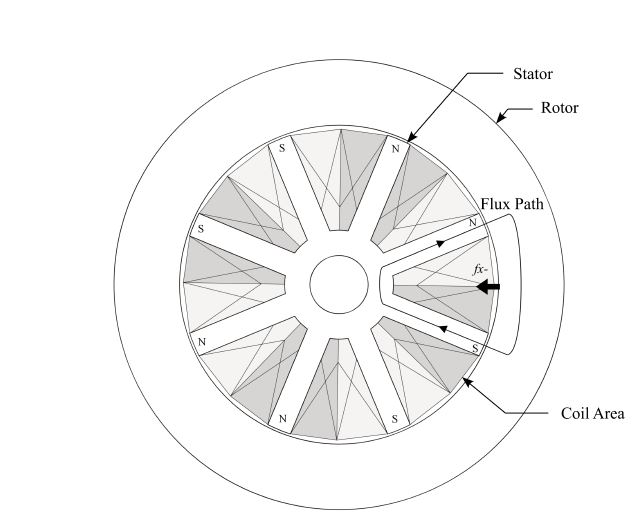
\includegraphics[width=4in]{./Pictures/StabB.jpg}
	\caption{UIFESS stabilization bearing configuration, from \cite{Kisling}}
	\label{fig:StabB}
\end{figure}

The magnetic circuit in Figure \ref{fig:SimpleMagneticCircuit} was created with the assumption that the horse shoe and floater are composed of iron. The assumptions that the two components are iron and that the permeability of iron is always much greater than 1 leads to the derivation presented in \cite{Wimer}. This derivation results in the simplification of equation \ref{Eq:BwFe} into equation \ref{Eq:BwoFe}. In the ensuing discussion, $ni$ or magnetomotive force (MMF) will be represented as $NI$.

\begin{figure}[!t]
	\centering
	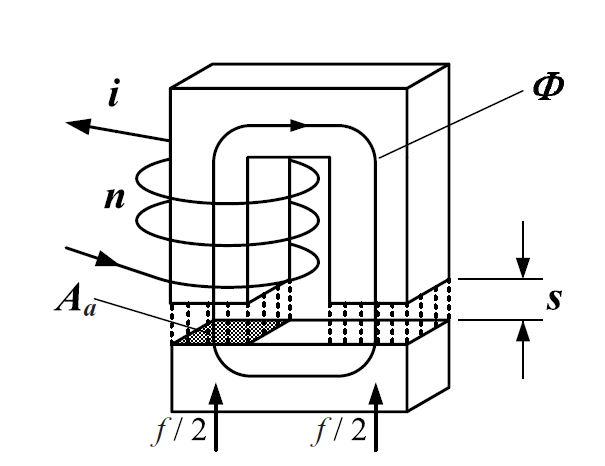
\includegraphics[width=4in]{./Pictures/SimpleMagneticCircuit.jpg}
	\caption{A simple magnetic circuit, from \cite{MagBear}}
	\label{fig:SimpleMagneticCircuit}
\end{figure}

\begin{equation}\label{Eq:BwFe}
	B={\mu }_{0}\frac{NI}{\Big(\frac{l_{fe}}{{\mu }_{r}}+2s\Big)}
\end{equation}

\begin{equation}\label{Eq:BwoFe}
	B={\mu }_{0}\frac{NI}{2s}
\end{equation}

If the horse shoe and the floater are not made of the same material then the equations needs to be modified starting with equation \ref{Eq:AmpLaw} where the floater is assumed to be made of a composite material. 

\begin{equation}\label{Eq:AmpLaw}
	\underset{l}{\oint }\stackrel{-}{H}\cdot d\stackrel{-}{s}={l}_{fe}{H}_{fe}+2s{H}_{a}+{l}_{c}{H}_{c}=NI
\end{equation}

Also assuming that the flux $\Phi$ follows a path within the magnetic loop and that the cross sections of each material are equal, the flux density $B$ can be computed from the following equations \cite{MagBear}. Where

\begin{equation}\label{Eq:flux}
	\Phi={A}_{fe}{B}_{fe}={A}_{a}{B}_{a}={A}_{c}{B}_{c}
\end{equation}
and
\begin{equation}\label{Eq:area}
	{A}_{fe}={A}_{a}={A}_{c}
\end{equation}
therefore
\begin{equation}\label{Eq:Beq}
	{B}_{fe}={B}_{a}={B}_{c}=B
\end{equation}

% ADD DISCUSSION ABOUT THE EFFECTS OF leakage flux


Since the flux density is identical in each of the materials, the field intensities ${H}_{fe}$, ${H}_{a}$, and ${H}_{c}$ from equation \ref{Eq:AmpLaw} can be replaced as shown in equation \ref{Eq:MMFwB}:

\begin{equation}\label{Eq:MMFwB}
	{l}_{fe}\frac{B}{{\mu}_{0}{\mu}_{fe}}+2s\frac{B}{{\mu}_{0}}+{l}_{c}\frac{B}{{\mu}_{0}{\mu}_{c}}=NI
\end{equation}

Solving equation \ref{Eq:MMFwB} for $B$ yields

\begin{equation}\label{Eq:B}
	B={\mu}_{0}\frac{NI}{\Big(\frac{{l}_{fe}}{{\mu}_{fe}}+2s+\frac{{l}_{c}}{{\mu}_{c}}\Big)}
\end{equation}

At this point it is useful to define a corrective term that can be used later. From equation \ref{Eq:B} it is clear that $B$ with a composite in the loop is equivalent to $B$ with only iron and air in the loop multiplied by a composite loss factor $k_{comp}$ defined below. This will be particularly useful when the calculation of MMF is complicated, such as is the case when using the modified winding approach, as the MMF can be calculated for an ideal case and corrected to include the composite by the application of the composite loss factor.

\begin{equation}\label{Eq:Kc}
	k_{comp}=\frac{\left(\frac{{l}_{fe}}{{\mu}_{fe}}+2s\right)}{\left(\frac{{l}_{fe}}{{\mu}_{fe}}+2s+\frac{{l}_{c}}{{\mu}_{c}}\right)}
\end{equation}

% ADD DISCUSSION ABOUT THE EFFECTS OF SATURATION ON B

The attraction force of an electromagnet is generated at the boundaries between differing permeability and can be calculated based on the field energy \cite{MagBear}.  The energy stored in the volume of the air gap can be expressed as

\begin{equation}\label{Eq:Wa}
	{W}_{a}=\frac{1}{2}{B}_{a}{H}_{a}{V}_{a}=\frac{{{B}_{a}}^{2}{V}_{a}}{2{\mu}_{0}}
\end{equation}
where
\begin{equation}\label{Eq:Va}
	{V}_{a}=2s{A}_{a}
\end{equation}

The force acting on the floater is generated by a change in the air gap field energy. This can be expressed as a function of the floater displacement. If the displacement is small the magnetic flux remains constant and an increase in displacement will result in an increase in energy \cite{MagBear}. Using the principle of virtual displacement, where the system is frozen in time and one degree of freedom is displaced by a small amount \cite{AnaMech}, the force can be expressed as the partial derivative of the field energy with respect to the air gap \cite{MagBear}.

\begin{equation}\label{Eq:F}
	f=-\frac{\partial {W}_{a}}{\partial s}=\frac{{{B}_{a}}^{2}{A}_{a}}{{\mu}_{0}}
\end{equation}

By combining equation \ref{Eq:F} and equation \ref{Eq:B}, the force on the floater can be expressed as a function of the coil current and air gap.

\begin{equation}\label{Eq:Fwis}
	f={\mu}_{0}{A}_{a}{\left[\frac{NI}{\Big(\frac{{l}_{fe}}{{\mu}_{fe}}+2s+\frac{{l}_{c}}{{\mu}_{c}}\Big)}\right]}^{2}
\end{equation}

This function is useful for the horse shoe configuration shown in Figure \ref{fig:SimpleMagneticCircuit} but needs to be modified for use with a cylindrical configuration as would be used with a machine. For a curved surface, like the one shown in Figure \ref{fig:CurvedMagneticCircuit},  $A_a$ is assumed to be the projected area of the pole face \cite{MagBear}. Also the angel $\alpha$ must be considered in determining the force and is dependent on the number of poles the machine has. Equation \ref{Eq:Fwis} can be modified with these considerations to produce:

\begin{figure}[h]
	\centering
	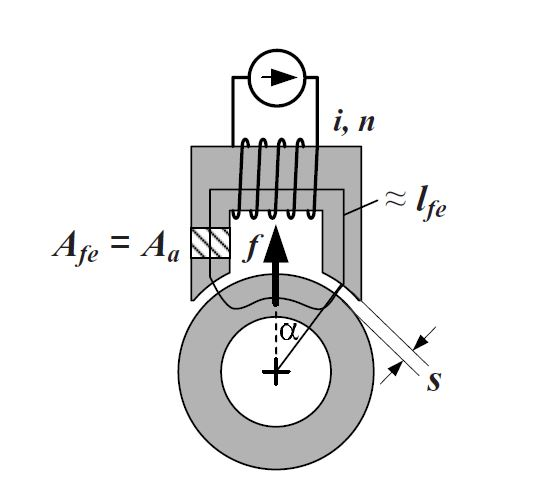
\includegraphics[width=4in]{./Pictures/CircularMagneticCircuit.jpg}
	\caption{A cylindrical magnetic circuit, from \cite{MagBear}}
	\label{fig:CurvedMagneticCircuit}
\end{figure}

\begin{equation}\label{Eq:FwisAlpha}
	f={\mu}_{0}{A}_{a}{\left[\frac{NI}{\Big(\frac{{l}_{fe}}{{\mu}_{fe}}+2s+\frac{{l}_{c}}{{\mu}_{c}}\Big)}\right]}^{2}\cos(\alpha)
\end{equation}

% ADD discussion on linearization and control 

% ADD discussion on magnetic equivalent circuits 

For this model to be used in the future of the UIFESS it needs to be both verified and validated. Verification of the model was performed by using another magnetic circuit modeling technique to determine whether the results are appropriate under the assumptions made. The modeling technique used is the gyrator-capacitor model developed by Buntenbach in the late 1960's. This technique uses MMF ($\mathcal{F}$) as a effort variable and rate of change of flux ($\frac{d\Phi }{dt}\equiv\stackrel{.}{\Phi}$) as a flow variable. Under this variable scheme magnetic permeance ($\mathcal{P}$) is analogous to electrical capacitance, and can be calculated using equation \ref{Eq:Perm}, where $A$ is cross section area and $\ell$ is member length \cite{GyrCapApp}.

\begin{equation}\label{Eq:Perm}
	\mathcal{P}={\mu}_{0}{\mu}_{r}\frac{A}{\ell}
\end{equation}

\begin{figure}[t]
	\centering
	\begin{picture}(150,240)
	\put(0,0){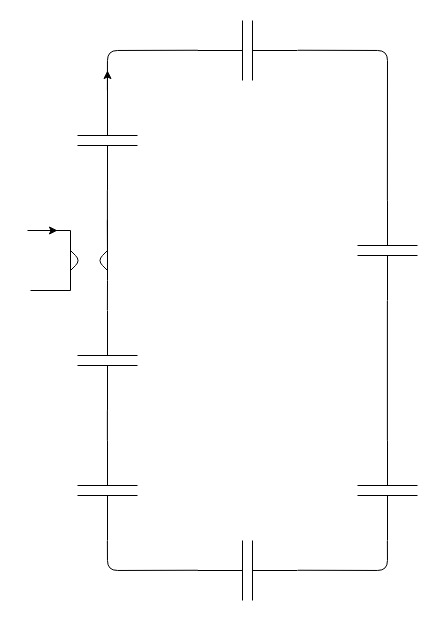
\includegraphics[width=2in]{./Pictures/Gyrator-CapApp.jpg}}
	\put(25,171){$\stackrel{.}{\Phi}$}
	\put(36,148){$\mathcal{P}_{fe1}$}
	\put(24,130){$N$}
	\put(12,130){$i$}
	\put(36,125){$+$}
	\put(36,115){$\mathcal{F}$}
	\put(36,107){$-$}
	\put(0,125){$+$}
	\put(0,115){$v$}
	\put(0,107){$-$}
	\put(36,75){$\mathcal{P}_{fe2}$}
	\put(36,32){$\mathcal{P}_{a}$}
	\put(85,8){$\mathcal{P}_{c}$}	
	\put(130,32){$\mathcal{P}_{a}$}		
	\put(130,112){$\mathcal{P}_{fe3}$}
	\put(85,180){$\mathcal{P}_{fe4}$}			
	\end{picture}
	\caption{A gyrator-capacitor model of a simple magnetic circuit}
	\label{fig:GyratorCapModel}
\end{figure}

The magnetic circuit shown in Figure \ref{fig:SimpleMagneticCircuit} can be represented as the gyrator-capacitor model shown in Figure \ref{fig:GyratorCapModel}. Where $\mathcal{P}_{fe}$, $\mathcal{P}_{a}$, and $\mathcal{P}_{c}$ are the permeance of iron, air, and a composite respectively. A distinct feature of this approach is that windings are treated as two port elements linking the electrical and magnetic circuits \cite{GyrCapApp}. The gyrator can be described using the following equations:

\begin{equation}\label{Eq:GyrV}
	v=N\stackrel{.}{\Phi}
\end{equation}

\begin{equation}\label{Eq:GyrI}
	i=\frac{\mathcal{F}}{N}
\end{equation}

Once the model is generated it can be analyzed as a capacitive circuit. In order to verify the force model represented in equation \ref{Eq:Fwis} the energy stored in the two $\mathcal{P}_{a}$ capacitors must be calculated, this represents the air gap energy. The energy stored in the air gap capacitor can be calculated using equation \ref{Eq:CapW}, where $\mathcal{F}_{a}$ is the MMF across the air gap.

\begin{equation}\label{Eq:CapW}
	W_{a}=\frac{1}{2}\mathcal{P}_{a}{\mathcal{F}_{a}}^{2}
\end{equation}

Equation \ref{Eq:CapW} requires the calculation of the MMF across the air gap:

\begin{equation}\label{Eq:CapV}
	\mathcal{F}_{a}=\frac{1}{\mathcal{P}_{a}}\left[{\int}_{{t}_{0}}^{\tau }\stackrel{.}{\Phi}dt+\mathcal{F}_{a0}\right]
\end{equation}

Then the force can be calculated by taking the partial derivative of the air gap energy with respect to the change in the air gap. Unfortunately this model does not reduce to a simple equation that represents the force as a function of the air gap and current. The model can be solved using a variety of softwares such as LTSpice\textsuperscript{\textregistered} or MATLAB\textsuperscript{\textregistered}. 

% ADD Discussion on the results of the two models

% ADD Discussion on the need for validation

% ADD Discusion on the benefits of each model.	

\section{Effects of Non Ideal Materials on the Drive Bearing}

The drive bearing of the machine, shown in Figure \ref{fig:DriveB}, has a more complicated configuration than the stabilization bearing. This configuration benefits from the use of modified winding theory, explained in detail in \cite{Wimer}. The derivation in \cite{Wimer} makes use of Ampere's law and assumes the components are iron and air, but can be modified to include the effect of the path $bc$, shown in Figure \ref{fig:SalientPole}, to account for a non ideal rotor material. 

\begin{figure}[h]
	\centering
	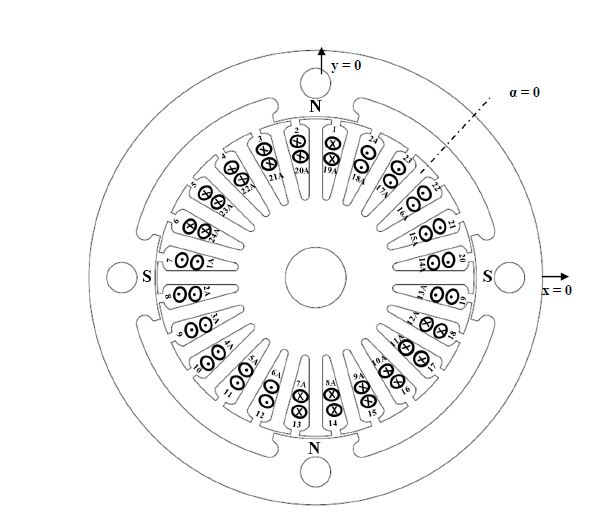
\includegraphics[width=4in]{./Pictures/DriveB.jpg}
	\caption{UIFESS drive bearing winding schematic, from \cite{Wimer}}
	\label{fig:DriveB}
\end{figure}

Ampere's law can be expressed as a series of $\mathcal{F}$ drops along the path $abcda$:

\begin{equation}\label{Eq:MMFdrops}
	\mathcal{F}_{ab}+\mathcal{F}_{bc}+\mathcal{F}_{cd}+\mathcal{F}_{da}=n(\phi)i
\end{equation}
where $n(\phi)$ is the turns function. The turns function represents the total number of turns enclosed by the path $abcda$ \cite{Wimer}. 

To include the effects of the non ideal rotor material the composite loss factor $k_{comp}$ needs to be configured as a function of $\phi$, where $\phi$ is the angle represented in Figure \ref{fig:SalientPole}. 

\begin{equation}\label{Eq:KcwP}
	k_{comp}(\phi)=\frac{\left(\frac{{l}_{fe}}{{\mu}_{fe}}+s({\phi}_{0})+s(\phi)\right)}{\left(\frac{{l}_{fe}}{{\mu}_{fe}}+s({\phi}_{0})+s(\phi)+\frac{{\int}_{{\phi}_{0}}^{\phi}\left(\sqrt{1+{{l}_{c}'(\varphi)}^{2}}\right)d\varphi}{{\mu}_{c}}\right)}
\end{equation}

\begin{figure}[!t]
	\centering
	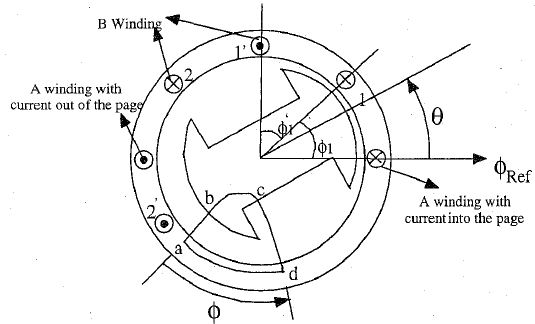
\includegraphics[width=4in]{./Pictures/SalientPole.jpg}
	\caption{A Salient-Pole Machine with Rotor Eccentricities, from \cite{MWFwE}}
	\label{fig:SalientPole}
\end{figure}

The composite loss factor can be further simplified by referring the effect of iron to the air gap. This is done by defining an effective air gap. This should be taken into account since the gap length $s$ is very small compared to the length of iron in the flux path. The effective air gap can be found by \cite{IntACMach}:

\begin{equation}\label{Eq:EqGap}
	{s}_{e}=\frac{{\mu}_{0}{\uptau}_{s}{l}_{e}}{\mathcal{P}_{s}}
\end{equation}
where ${\uptau}_{s}$ is the slot pitch width and ${l}_{e}$ is the height of the machine. From the effective air gap a Carter factor can be defined as \cite{IntACMach}:
\begin{equation}\label{Eq:Cfac}
	{s}_{e}={k}_{c}s
\end{equation}
and by combining equations \ref{Eq:EqGap} and \ref{Eq:Cfac} we can calculate the Carter factor as
\begin{equation}\label{Eq:CfacwP}
	{k}_{c}=\frac{{\mu}_{0}{\uptau}_{s}{l}_{e}}{\mathcal{P}_{s}}s
\end{equation}

This representation allows the calculation of the Carter factor to be split into two components. One to represent the effect of the stator slots and teeth. Another component of the Carter factor represents the effect of the salient poles of the rotor.

\begin{equation}\label{Eq:Cfacwrs}
	{k}_{c}={k}_{cs}{k}_{cr}
\end{equation}

In order to determine the Carter factor, and consequently the effective air gap, the permeance of the air gap due to the slot openings and due to the salient pole are needed. There are different analytical approaches to calculate the air gap permeance in electrical machines. In \cite{AnaGapSal}, a method of analytically determining the air gap permeance due to both the slot opening and salient poles is presented. This method is described by the equations below and referring to Figure \ref{fig:Perm}.

For the effective permeance of the stator slots and teeth the effective slot width ${b}_{0}'$, shown in Figure \ref{fig:Perm} (a), needs to be considered. In this case the air gap permeance is constant within the reduced tooth width ${\uptau }_{s}' - {b}_{0}'$ \cite{AnaGapSal}.
The permeance of the half close slots is calculated using the Fourier decomposition:
\begin{equation}\label{Eq:SOGPermas}
	\mathcal{P}_{s,a}(\gamma') = \mathcal{P}_{smin,a0} + \sum_{v'}\mathcal{P}_{smin,av'}\cos\left(v'\gamma'\right)
\end{equation}
\hspace{1in}where
\begin{equation}\label{Eq:SOGPermsmina0}
	\mathcal{P}_{smin,a0} = \frac{{\mu}_{0}}{\delta} \left[1 - \beta\frac{{b}_{0}'}{{\uptau }_{s}'}\right]
\end{equation}
\hspace{1in}and
\begin{equation}\label{Eq:SOGPermsminav}
	\mathcal{P}_{smin,av'} = \frac{{\mu}_{0}}{\delta} \frac{\beta{N}}{v'\pi} \frac{2}{ \left(\frac{v'{b}_{0}'}{2\pi}\right)^{2} - 1} \sin\left(\frac{v'{b}_{0}'}{2}\right)
\end{equation}

The permeance of the open slots is calculated using the Fourier decomposition:
\begin{equation}\label{Eq:SOGPermbs}
	\mathcal{P}_{s,b}(\gamma') = \mathcal{P}_{smin,b0} + \sum_{v'}\mathcal{P}_{smin,bv'}\cos\left(v'\gamma'\right)
\end{equation}
\hspace{1in}where
\begin{equation}\label{Eq:SOGPermsminb0}
	\mathcal{P}_{smin,b0} = \frac{{\mu}_{0}}{\delta} \left[1 - \frac{11}{8}\beta\frac{{b}_{0}'}{{\uptau }_{s}'}\right]
\end{equation}
\hspace{1in}and
\begin{equation}\label{Eq:SOGPermsminbv}
	\mathcal{P}_{smin,bv'} = \frac{{\mu}_{0}}{\delta} \frac{\beta{N}}{8v'\pi} \left[\frac{15}{1 - \left(\frac{2\pi}{v'{b}_{0}'}\right)^{2}} + \frac{6}{1 - 4\left(\frac{2\pi}{v'{b}_{0}'}\right)^{2}} + \frac{1}{1 - 9\left(\frac{2\pi}{v'{b}_{0}'}\right)^{2}} - 22\right] \sin\left(\frac{v'{b}_{0}'}{2}\right)
\end{equation}

The amplitudes belonging to the air gap permeance due to the slot openings of the stator comply with the condition \cite{AnaGapSal}:

\begin{equation}\label{Eq:v}
	v' = {g}_{1}N \wedge {f}_{v'} = 0 \:\:\: \:\forall\: {g}_{1} \in \mathbb{N}_{0}
\end{equation}

The term $N$ is the number of stator slots, and the term $\beta$ is the drop of the magnetic field density in the middle of the slots. The functions also require the effective slot width ${b}_{0}'$.

\begin{equation}\label{Eq:Beta}
	\beta = \frac{1}{2} - \frac{1}{\sqrt{4 + \left(\frac{{b}_{s}}{\delta}\right)^{2}}}
\end{equation}

\begin{equation}\label{Eq:EffSlotw}
	{b}_{0}' = {b}_{s}'\left(1 + \left[0.8 + 10^{-4}\left(\frac{{b}_{s}}{\delta} - 6 \right)^{4} \right] \exp\left(-\frac{1}{8.5}\left(\frac{{b}_{s}}{\delta}-0.9\right)\right) \right)
\end{equation}

Finally the two portions of the permeance can be combined with the weighting factor $a$ to determine the total effective air gap permeance of the stator slots and teeth.

\begin{equation}\label{Eq:SOGPerm}
	\mathcal{P}_{s}(\gamma') = a\mathcal{P}_{s,a}(\gamma') + (1-a)\mathcal{P}_{s,b}(\gamma')
\end{equation}

\begin{equation}\label{Eq:SOGPerma}
	a =
	\begin{cases} 
		\exp\left( -\frac{1}{6} \left(\frac{{b}_{s}}{\delta} - 1 \right)\right) & \forall \:  \frac{{b}_{s}}{\delta} \geq 10.6 \\
		\sin^{4}\left(\frac{\pi}{2}\frac{19 - \frac{{b}_{s}}{\delta}}{18}\right) & \forall \: \frac{{b}_{s}}{\delta} < 10.6 \\
	\end{cases}
\end{equation}

For a rotor with a curved pole the process of determining the effective permeance of the salient pole needs to consider the non uniform air gap \cite{AnaGapSal}. This geometry is represented in Figure \ref{fig:Perm} (c). The non uniform air gap dictates the need to define a function to calculate the air gap length:
\begin{equation}\label{Eq:dofgamma}
	\delta({\gamma}_{fd}') = R_{i} - \sqrt{{R}_{PS}^{2} + {I}_{m}^{2} - 2{R}_{PS}{I}_{m}\cos\left(\pi - {\gamma}_{fd}' - {\gamma}^{\star} \right)}
\end{equation}
\hspace{1in}where
\begin{equation}\label{Eq:gammastar}
	{\gamma}^{\star} = \arcsin\left[\frac{{I}_{m}\sin\left({\gamma}_{fd}'\right)}{{R}_{PS}}\right]
\end{equation}
\hspace{1in}and
\begin{equation}\label{Eq:Im}
	{I}_{m} = {R}_{i} - {\delta}_{0} - {R}_{PS}
\end{equation}

The effective pole shoe width can be defined as ${b}_{P0}'$ which is based on finite element method data calculated for various rotor pole geometries \cite{AnaGapSal}.
 
\begin{equation}\label{Eq:bpo}
	{b}_{P0}' = 0.9\alpha{\uptau}_{p}
\end{equation}

\begin{equation}\label{Eq:Permin}
	{\mathcal{P}}_{min,PG} = \frac{{\mu}_{0}}{{\delta}_{0}}\left(1 - 2{\beta}_{PG}\right)
\end{equation}

\begin{equation}\label{Eq:Betapg}
	{\beta}_{PG} = \frac{1}{2} - \frac{1}{\sqrt{4 + \left(\frac{{b}_{SP}}{{\delta}_{0}}\right)^{1.685}}}
\end{equation}

\begin{equation}\label{Eq:bsp}
	{b}_{SP} = \left(1 - \alpha\right){\uptau}_{p}'\left({R}_{i} - {\delta}_{0}\right)
\end{equation}

\begin{equation}\label{Eq:SPGPermas}
	\mathcal{P}_{sp,a}({\gamma}_{fd}') = 
	\begin{cases}
		\frac{{\mu}_{0}}{\delta(-\frac{{b}_{P0}'}{2})} \left[ 1 - \beta{x}_{a2} \right] & \forall \: -\frac{{\uptau}_{p}'}{2} < {\gamma}_{fd}' < -\frac{{b}_{P0}'}{2} \\ 
		\frac{{\mu}_{0}}{\delta({\gamma}_{fd}')} & \forall \: -\frac{{b}_{P0}'}{2} < {\gamma}_{fd}' < \frac{{b}_{P0}'}{2} \\
		\frac{{\mu}_{0}}{\delta(\frac{{b}_{P0}'}{2})} \left[ 1 - \beta{x}_{a1} \right] & \forall \: \frac{{b}_{P0}'}{2} < {\gamma}_{fd}' < \frac{{\uptau}_{p}'}{2} \\
	\end{cases}
\end{equation}

\begin{equation}\label{Eq:SPGPermax1}
	{x}_{a1} = 1 + \cos\left(\frac{2\pi}{{b}_{G0}'} \left({\gamma}_{fd}' - \frac{{\uptau}_{p}'}{2}\right) \right)
\end{equation}

\begin{equation}\label{Eq:SPGPermax2}
	{x}_{a2} = 1 + \cos\left(\frac{2\pi}{{b}_{G0}'} \left({\gamma}_{fd}' + \frac{{\uptau}_{p}'}{2}\right) \right)
\end{equation}

\begin{equation}\label{Eq:BetaSP}
	{\beta}_{SP} = \frac{1}{2} \left(1 - \frac{{\mathcal{P}}_{min,PG}}{\frac{{\mu}_{0}}{{\delta}({\gamma}_{fd}')}}\right)
\end{equation}

\begin{equation}\label{Eq:bg0}
	{b}_{G0}' = {\uptau}_{p}' - {b}_{P0}'
\end{equation}

\begin{equation}\label{Eq:SPGPermbs}
	\mathcal{P}_{sp,b}({\gamma}_{fd}') = 
	\begin{cases}
		\frac{{\mu}_{0}}{\delta(-\frac{{b}_{P0}'}{2})} \left[ 1 - 2\beta{x}_{b2} \right] & \forall \: -\frac{{\uptau}_{p}'}{2} < {\gamma}_{fd}' < -\frac{{b}_{P0}'}{2} \\ 
		\frac{{\mu}_{0}}{\delta({\gamma}_{fd}')} & \forall \: -\frac{{b}_{P0}'}{2} < {\gamma}_{fd}' < \frac{{b}_{P0}'}{2} \\
		\frac{{\mu}_{0}}{\delta(\frac{{b}_{P0}'}{2})} \left[ 1 - 2\beta{x}_{b1} \right] & \forall \: \frac{{b}_{P0}'}{2} < {\gamma}_{fd}' < \frac{{\uptau}_{p}'}{2} \\
	\end{cases}
\end{equation}

\begin{equation}\label{Eq:SPGPermbx1}
	{x}_{b1} = 1 + \cos\left(\frac{2\pi}{{b}_{G0}'} \left({\gamma}_{fd}' - \frac{{\uptau}_{p}'}{2}\right) \right)
\end{equation}

\begin{equation}\label{Eq:SPGPermbx2}
	{x}_{b2} = 1 + \cos\left(\frac{2\pi}{{b}_{G0}'} \left({\gamma}_{fd}' + \frac{{\uptau}_{p}'}{2}\right) \right)
\end{equation}

\begin{equation}\label{Eq:SPGPerm}
	\mathcal{P}_{sp}({\gamma}_{fd}') = a\mathcal{P}_{sp,a}({\gamma}_{fd}') + (1-a)\mathcal{P}_{sp,b}({\gamma}_{fd}')
\end{equation}

\begin{equation}\label{Eq:SPGPerma}
	a_{sp} = 5\alpha^{2} - 3.97\alpha + 0.6135
\end{equation}

The configuration of the UIFESS results in a simplification of the salient pole section represented in Figure \ref{fig:Perm} (b) and (c). This simplification results in the rotor portion of the air gap permeance being calculated like that of the stator slot portion of the air gap permeance. The curved rotor pole equations \ref{Eq:dofgamma} - \ref{Eq:SPGPerma} are included for future reference in the event that a curved rotor pole topology is used in the future designs of the device. 

\begin{figure}[!t]
	\begin{subfigure}{0.5\textwidth}
		\centering
		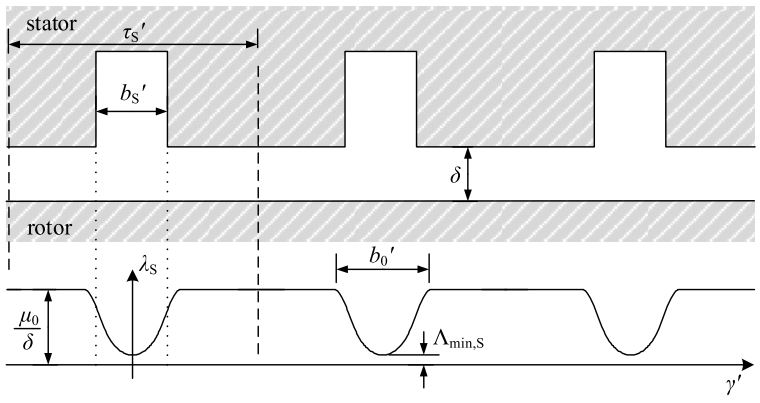
\includegraphics[width=3in]{./Pictures/SlotPerm.jpg}
		\caption{}
	\end{subfigure}
	\begin{subfigure}{0.5\textwidth}
		\centering
		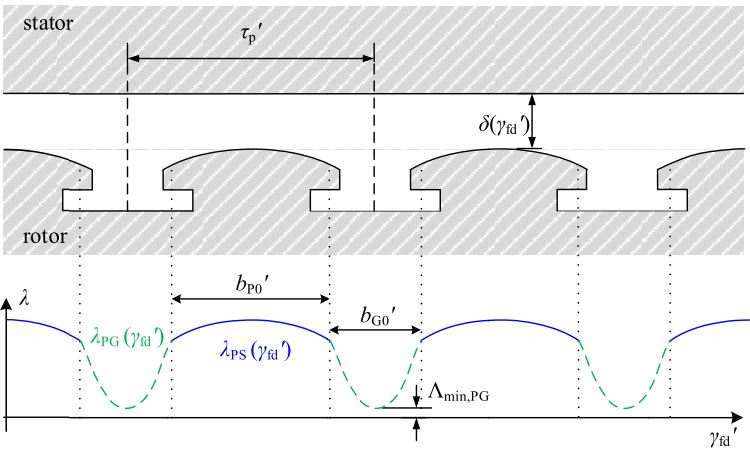
\includegraphics[width=2.6in]{./Pictures/PolePerm.jpg}
		\caption{}
	\end{subfigure}
	\begin{subfigure}{\textwidth}
		\centering
		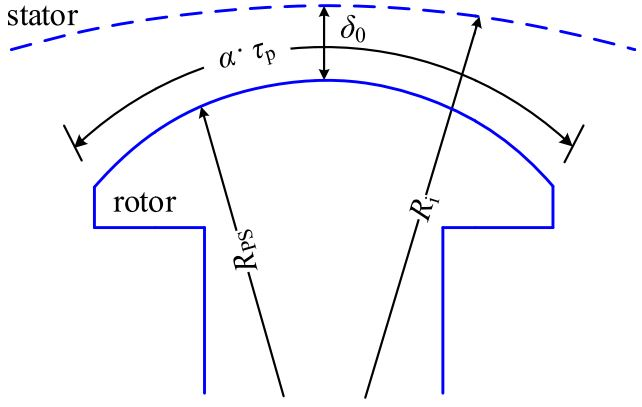
\includegraphics[width=3in]{./Pictures/SalientGeom.jpg}
		\caption{}
	\end{subfigure}
	\caption{(a) Air gap permeance due to slot openings, (b) Air gap permeance due to pole gaps, and (c) Geometry of a salient pole, from \cite{AnaGapSal}}
	\label{fig:Perm}
\end{figure}


%\begin{figure}[h]
%	\centering
%	\subfloat{
%		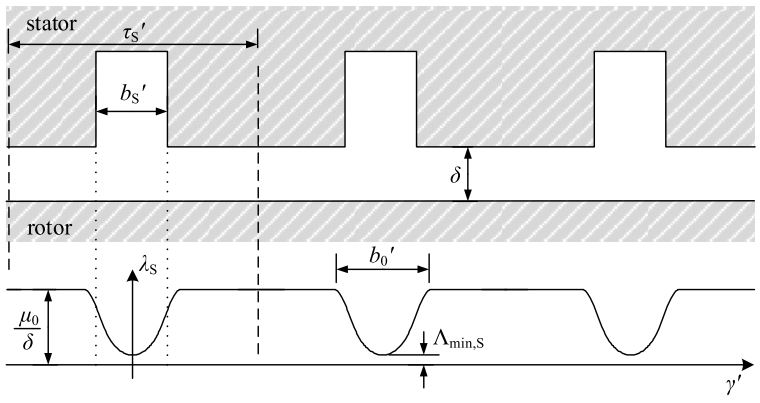
\includegraphics[width=0.5\textwidth]{./Pictures/SlotPerm.jpg}
%		\label{fig:subfig1}}
%	\qquad
%	\subfloat{
%		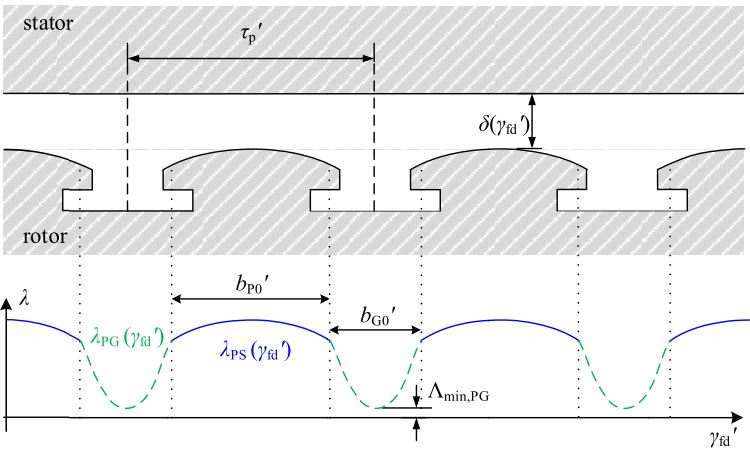
\includegraphics[width=0.4\textwidth]{./Pictures/PolePerm.jpg}
%		\label{fig:subfig2}}
%	\subfloat{
%		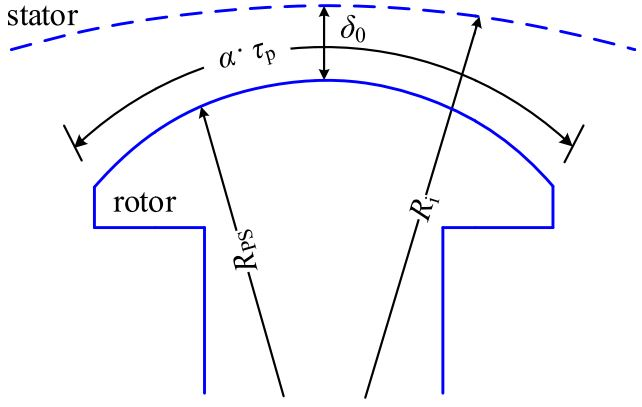
\includegraphics[width=0.4\textwidth]{./Pictures/SalientGeom.jpg}
%		\label{fig:subfig3}}
%	\qquad
%	\caption{(a) Air gap permeance due to slot openings, (b) Air gap permeance due to pole gaps, and (c) Geometry of a salient pole, from \cite{AnaPermSalient}
%	\label{fig:globfig}
%\end{figure}



\section{Torque Production}


The torque production in the model is determined by taking the derivative of the air gap energy with respect to the displacement angle.

% ADD Discussion on the effects of saturation

% ADD Discussion on the effects of non ideal materials



\section{MATLAB\textsuperscript{\textregistered} Development}
Pain in my ass

	
	\chapter{Controls Development}
	%\input{chapters/AMB_Control_System}
	
	\chapter{Hardware Testing}
	%\input{chapters/SASB_Test_Setup}
	
	\chapter{Model Validation and Verification}
	%\input{chapters/Stabilization_Bearing_Design}
	
	\chapter{Summary, Conclusions, and Recommendations}
	%\input{chapters/Rec_for_Future_Work}
	
	\renewcommand{\bibname}{References} %Change name from "Bibliography" to "References"
	\setlength{\bibitemsep}{1cm}        %Set spacing between bibliography entries       
	\cleardoublepage
	\phantomsection
	\addcontentsline{toc}{chapter}{References}
	% \let\itshape\upshape
	\urlstyle{same}
	\uspunctuation
	\printbibliography
	
	
	%\appendix
	%\chapter{My First Appendix}
	%\input{chapters/appendix_1}
	
	
	%\includepdf[pages={1}]{test_pdf_file.pdf}
	%\includepdf[pages=-,scale=.8,pagecommand={}]{test_pdf_file.pdf}
\end{document}


